In this section explains required the theoretical background and context for this thesis. First introducing fundamental concepts of software development, the agile software development lifecycle (SDLC), Continuous Integration (CI), and software project hosting platforms. The second part explores Generative Ai and LLMs with their rising role in software development practices. The third part explores the evolution and state of Automated Program Repair (APR) with examples of existing approaches.

\section{Software Development}

The following section introduces core concepts of software development starting with the software development lifecycle followed by importance of Continuous Integration (CI) in modern software development and the role of software project hosting platforms.

\subsection{Software Development Lifecycle}
%TODO add tickets that are created by developers, product managers, ...
Engineering and developing software is complex process, consisting of multiple different tasks. For structuring this process, software development lifecycle models have been introduced. These frameworks evolve constantly to adapt to the changing needs of creating software. One of the most promising and widely used model today is Agile \cite{rupareliaSoftwareDevelopmentLifecycle2010, abrahamssonAgileSoftwareDevelopment2017}.

The Agile lifecycle introduces an iterative approach to software development, focusing on collaboration, feedback and adaptivity. The Goal is frequent delivery of small functional features of software, allowing for continuous improvement and adaptation to changing requirements \cite{rupareliaSoftwareDevelopmentLifecycle2010, abrahamssonAgileSoftwareDevelopment2017}. Agile frameworks like Scrum or Kanban are used to apply this approach in a development environment \cite{zayatFrameworkStudyAgile2020}.

An Agile iteration consists of multiple stages. Figure \ref{fig:agile-cycle} shows an example an agile iteration interpretation. Iterations start with a planning phase where requirements are gathered and prioritized. Secondly the architecture and design of the required changes is constructed in the design phase. The third stage is where the development of the prioritized requirements takes place. After development the changes are tested for issues or bugs in the testing stage. On successful integration and testing the changes are released in the deployment stage. Finally, internal and user feedback is collected for review \cite{huoSoftwareQualityAgile2004}.

\begin{figure}[H]
    \centering
    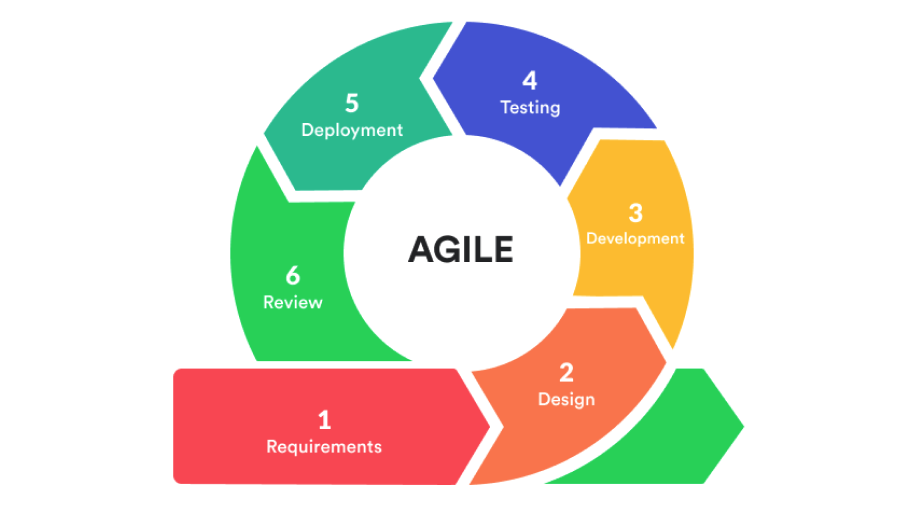
\includegraphics[width=1\textwidth]{images/agile-cycle.png}
    \caption{Agile software development lifecycle}
    \label{fig:agile-cycle}
\end{figure}


When bugs arise during an iteration requirements can be reprioritized and the iteration can be adapted to fix these issues. This adaptivity is a key feature of Agile software development, allowing teams to respond quickly to changing requirements and issues which can slows down delivery of planed features %\cite{}. %TODO how do i cite this?

Modern software systems are moving towards lightly coupled microservice architectures, which results in more repositories which are smaller in scale tailored towards a specialized domain. This trend is driven by the need for flexibility, scalability, and faster development cycles. This approach aligns with modern agile software development practices. \cite{francescoResearchArchitectingMicroservices2017} Along with this trend developers tend to work on multiple projects at the same time, which can lead to more interruptions and context switching when problems arise and priorities shift. \cite{tregubovImpactTaskSwitching2017, vasilescuSkyNotLimit2016}

\subsection{Continuous Integration}

For accelerating development and delivery of software in an Continuous Integration has become a standard in agile software development. CI can  development and testing in the development lifecycle \cite{ugwuezeContinuousIntegrationDeployment2024}. It enables frequent code integration into a code repository. Automating steps like building and testing into the development resulting in rapid feedback right where the changes are committed. This supports critical aspects of agile software development enhancing delivery, feedback and collaboration  \cite{ugwuezeContinuousIntegrationDeployment2024}. Figure \ref{fig:ci-cycle} illustrates a typical CI cycle, where code changes are automatically fetched from source control, built, and tested, with a report generated for the developer.

\begin{figure}[H]
    \centering
    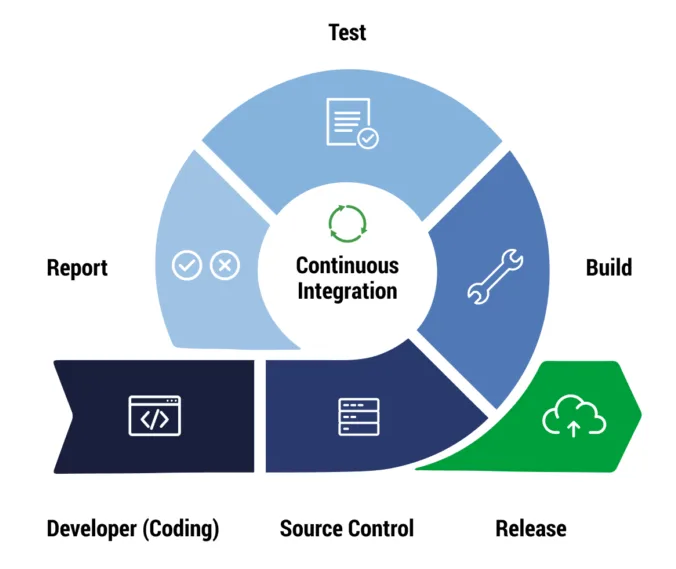
\includegraphics[width=1\textwidth]{images/ci-cycle.png}
    \caption{Continuous Integration cycle}
    \label{fig:ci-cycle}
\end{figure}

Although Continuous Integration improves feedback loops, can also add overhead. Effort and infrastructure needs to be invested tp keep pipelines running \cite{hiltonUsageCostsBenefits2016}, and projects suffer from long build times that harm developer productivity \cite{ghalebEmpiricalStudyLong2019}.

\subsection{Software Project Hosting Platforms} \label{subsection:Software Project Hosting Platforms}

Modern software projects live on platforms like Github or GitLab. GitHub alone   100 million developers and more than 518 million repositories, making it the largest open-source community world wide \cite{staffOctoverseAILeads2024}.

Development platforms offer tools and services for the entire software development lifecycle, including project hosting, version control, issue tracking, bug reporting, project management, backups, collaborative workflows, and documentation capabilities. \cite{GitHubFeatures2025, abrahamssonAgileSoftwareDevelopment2017}

Github issues are a key feature of Github allowing for project a scoped backlog, tracking tasks, features, and bugs. Issues can be created, assigned, labeled, and commented on by everyone working on a codebase. This feature provides a structured way to manage and prioritize work within a project \cite{Issues}. Figure \ref{fig:gh-issue} shows an example of a GitHub Issue.

\begin{figure}[H]
    \centering
    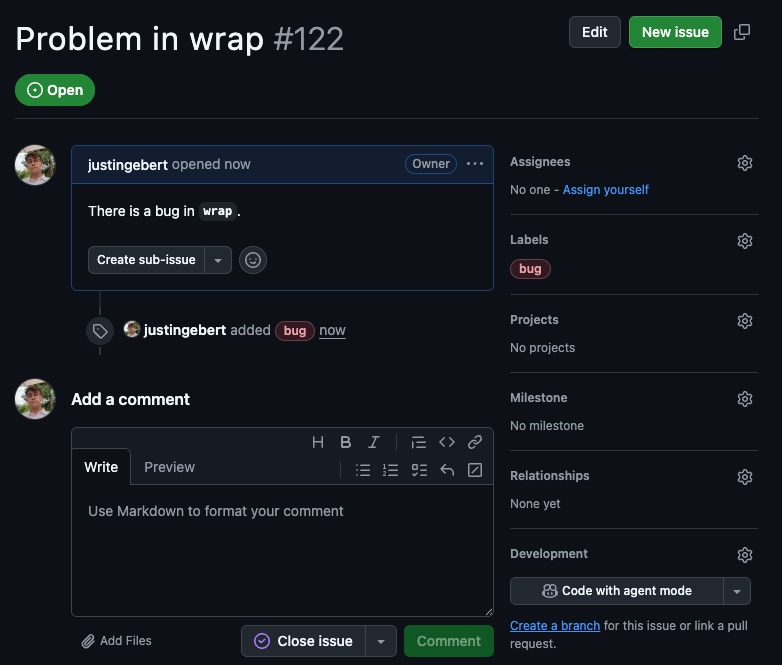
\includegraphics[width=1\textwidth]{images/github/github_issue.png}
    \caption{Example of a GitHub Issue}
    \label{fig:gh-issue}
\end{figure}

For integrating and reviewing code GitHub provides Pull Requests. A Pull Request proposes changes to the codebase, bringing along an integrated review process to validate changes before they are merged into the production codebase. Code changes are displayed in a diff format \footnote{TODO explain format} allowing reviewers to see and dig into the changes made. This process is essential for maintaining code quality and ensuring that changes are validated before being merged. Pull requests can be linked to Issues, allowing for easy tracking of changes related to specific tasks or bugs. \cite{PullRequests}

Moreover, GitHub also provides a manged solution (Github Actions) for running CI pipelines in a repositories. CI pipelines can be used by writing workflows files in YAML. Workflows can run self hosted or hosted by GitHub. A workflow consists of triggers and jobs, and steps. One or more events can trigger a workflow which executed one ore more jobs which are made up of one or more steps. \cite{UnderstandingGitHubActions} Figure \ref{fig:gh-workflow} visualizes the part of a workflow on GitHub.

\begin{figure}[H]
    \centering
    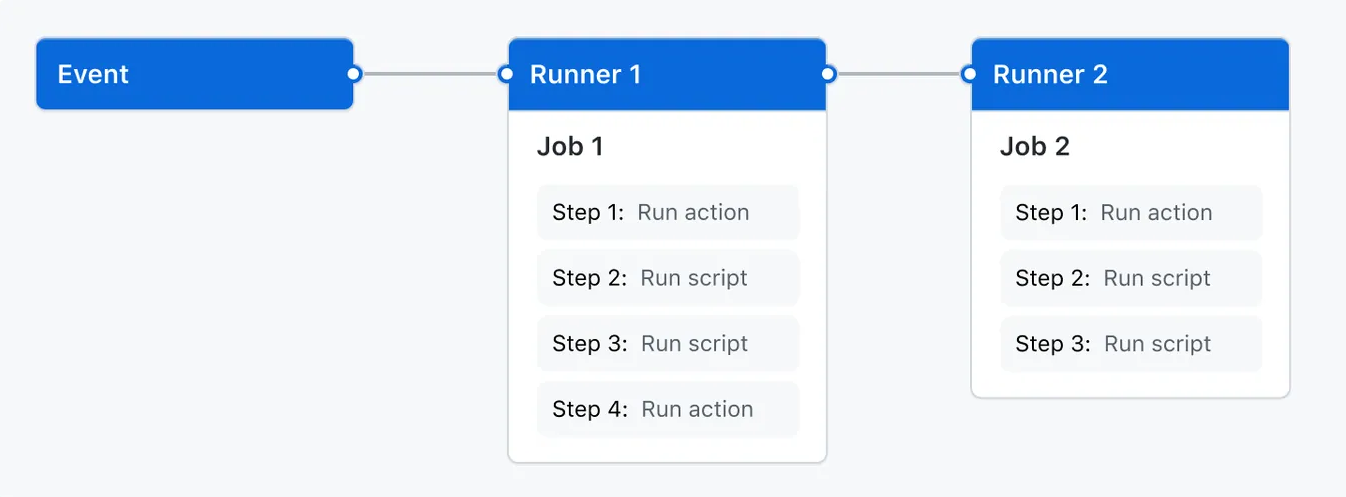
\includegraphics[width=1\textwidth]{images/overview-actions-simple.png}
    \caption{Components of a Github Action}
    \label{fig:gh-workflow}
\end{figure}

Workflow results and logs can be viewed from multiple places in the GitHub Web User Interface (UI), including the Actions tab, the Pull Request page, and the repository's main page. This integration provides a seamless experience for developers to monitor and manage their CI processes directly within their repositories. \cite{GitHubActions2025}

\section{Generative AI in Software Development}

This section will cover the role of Generative AI in modern software development. First we will define what Generative AI and Large Language Models (LLMs) are. The second part will focus on the impact of Generative AI on software development practices.

\subsection{Generative AI and Large Language Models}
%TODO add thinking definition of LLMS - and llms are few shot better than zero shot -> cite few shot learners paper
Generative Artificial Intelligence (GenAI) is subfield of artificial intelligence and refers to systems that can generate new content based on patterns learned from massive amounts of training data. Advanced machine learning techniques, particularly deep learning, enable these systems to generate text, images, or code, that resembles human generated output. \cite{WhatGenerativeAI2021}

The introduction of the transformer architecture revolutionized the field of text generation and natural language processing (NLP). This architecture laid the ground work for Large Language Models. \cite{changSurveyEvaluationLarge2024, naveedComprehensiveOverviewLarge2024} Extensive training, results in LLMs with billions of parameters, which allows them to understand and generate text in natural languages and diverse programming languages. Research has shown that a models sizes is a large factor of  its performance, with larger models generally achieving better results in various NLP tasks \cite{kaplanScalingLawsNeural2020}. However with larger models training and operating requires significant computational resources. \cite{LLMsWhatsLarge, naveedComprehensiveOverviewLarge2024}. Furthermore despite modern LLMs showing promising results in text generation, they can still hallucinate incorrect or biased content. \cite{LLMsWhatsLarge}.

To archive a specific task using LLMs, an input prompt given to a LLM. Designing these inputs to to guide a models output is called prompt engineering. This process is crucial for achieving desired results from LLMs, as the quality and specificity of the prompt directly influences the model's output. Text used for input and output of LLMs is tokenized, meaning that text is broken down into smaller units (tokens) for processing. The input is constrained by a models context window, which is the maximum amount of text the model can process at once. \cite{naveedComprehensiveOverviewLarge2024}

Large Language Models can be used via APIs offered by providers like OpenAI, Anthropic or Google. A selection of LLMs with characteristics is shown in section \ref{subsection:llm-selection}.

\subsection{Large Language Models in Software Development}

Large Language Models are reshaping software development by automating various tasks \cite{houLargeLanguageModels2024}. With billions of parameters and pre training on massive codebases these models show extraordinary capabilities in this area \cite{chenUnveilingPitfallsUnderstanding2025}. Tools like ChatGPT\footnote{link to gpt} and Github Copilot\footnote{link to copilot} have become popular in the software development community, providing developers with AI-powered code suggestions and completions \cite{bhargavmallampatiRoleGenerativeAI2025}. These tools get applied in various stages of the software development lifecycle, including requirement engineering, code generation, refactoring, testing and debugging. \cite{houLargeLanguageModels2024, puvvadiCodingAgentsComprehensive2025,bhargavmallampatiRoleGenerativeAI2025}. By using LLMs development cycle times can be reduced by up to 30 percent \cite{bhargavmallampatiRoleGenerativeAI2025,kalliamvakouResearchQuantifyingGitHub2022}. Furthermore these tools can have positive impacts, like improving developer satisfaction and reducing cognitive load \cite{kalliamvakouResearchQuantifyingGitHub2022}.

Despite Generative AI getting rapidly adopted in many areas of software development this technology still faces limitations. LLMs have challenges working on tasks that are outside their scope of training or require specific domain knowledge \cite{houLargeLanguageModels2024}. With limited context windows limitations arise when working with large codebases and complex projects where context windows are too small for true contextual or business requirement understanding \cite{bhargavmallampatiRoleGenerativeAI2025}. When generating code LLMs can produce incorrect or insecure code, which can lead to further bugs and vulnerabilities in the software \cite{houLargeLanguageModels2024, bhargavmallampatiRoleGenerativeAI2025}. Additionally when integrating LLMs, tools can become vulnerable to prompt injection, where malicious instructions are injected, which can lead to generation of harmful code \cite{liuPromptInjectionAttack2024}. Moreover, code generated by LLMs is based on existing data used for training. This raises questions about ownership, responsibility and intellectual property rights. \cite{sauvolaFutureSoftwareDevelopment2024, houLargeLanguageModels2024}.

Facing these challenges, different approaches are actively being developed and researched. For example AI Agents \cite{liuMarsCodeAgentAInative2024,yangSWEagentAgentComputerInterfaces2024}, Retrieval Augmented (RAG) approaches \cite{xiaAgentlessDemystifyingLLMbased2024} or interactive systems \cite{xiaAutomatedProgramRepair2024}. These paradigms aim to enhance the capabilities of LLMs by providing additional context, enabling multi step reasoning, or allowing for interactive feedback loops during code generation and debugging \cite{houLargeLanguageModels2024, puvvadiCodingAgentsComprehensive2025}. Section \ref{subsection:evolution-apr} deals with the mentioned approaches into more detail.

Recently research is exploring solutions which integration LLMs into existing software development practices and workflows. Leveraging existing development tools and platforms for integrating LLMs into the software development lifecycle. \cite{puvvadiCodingAgentsComprehensive2025, dohmkeGitHubCopilotMeet2025, IntroducingCodex, sauvolaFutureSoftwareDevelopment2024}

\section{Automated Program Repair}

Automated Program Repair (APR) is used to detect and repair bugs in code with minimal human intervention. \cite{zhangSurveyLearningbasedAutomated2024} APR systems are supposed to take over the process of fixing bugs, reducing load for developers and making time to focus on more relevant work. \cite{houLargeLanguageModels2024}

Using APR systems specific bugs can be fixed using a generated patch. Working patches are usually generated using a 3 stage approach: First localizing the bug. Then repairing the bug, in the end validation decides where the bug will be passed on \cite{zhangSurveyLearningbasedAutomated2024, baderGetafixLearningFix2019}. This approach is similar to the bug fixing process of a developer, where the bug is first identified, then fixed, and finally tested and reviewed to ensure the fix works as intended. An example of an APR system being applied at scale is Getafix, which is used at Meta to automatically fix common bugs in their production codebase \cite{baderGetafixLearningFix2019}.

The field of Automated program repair also greatly benefited of the rapid advancements in AI. With new research and benchmarks setting new standards in the field.\cite{puvvadiCodingAgentsComprehensive2025,houLargeLanguageModels2024}

In this section we will provide an overview of the evolution of APR, related work, and the current state of APR systems. Followed listing APR benchmarks which are used in APR research.

\subsection{Evolution of Automated Program Repair} \label{subsection:evolution-apr}

We have seen multiple paradigm shifts in the field of Automated Program Repair (APR) over the years. This evolution of APR can be categorized into key stages, each marked by significant advancements in techniques and methodologies.

\textbf{Traditional Approaches:}

Traditional APR approaches typically rely on manual crafted rules and predefined pattern. \cite{liuMarsCodeAgentAInative2024, xiaAutomatedProgramRepair2023,yinThinkRepairSelfDirectedAutomated2024}. These methods are generally classified into three main categories: search based, constraint/semantic based, and template-based repair techniques.
\begin{itemize}
    \item\textbf{Search based repair} searches for the correct predefined patch in a large search space. \cite{liuMarsCodeAgentAInative2024, huCanGPTO1Kill2024,zhangPATCHEmpoweringLarge2025} A popular example is GenProg, which uses genetic algorithms to evolve patches by mutating existing code and selecting based on fitness determined by test cases \cite{legouesGenProgGenericMethod2012}.

    \item\textbf{Semantics / constraint based repair} synthesizes patches using constraint solvers to based on semantic information of the program and tests. \cite{liuMarsCodeAgentAInative2024, mechtaevAngelixScalableMultiline2016} Angelix being a prominent example. \cite{mechtaevAngelixScalableMultiline2016}.

    \item\textbf{Template based repair} relies on mined templates for transformations of known bugs. \cite{xiaAutomatedProgramRepair2023} Templates are mined from previous human produced bug fixes.\cite{xiaAutomatedProgramRepair2023, yinThinkRepairSelfDirectedAutomated2024}. Getafix being an example of an industrially deployed tool learning recurring fix pattern form past fixes \cite{baderGetafixLearningFix2019}
\end{itemize}

Traditional systems face significant limitations in scalability and adaptability. They struggle to generalize to new and unseen bugs, or to adapt to evolving codebases. Often requiring extensive computational resources and manual effort. \cite{puvvadiCodingAgentsComprehensive2025, xiaAutomatedProgramRepair2024}


\textbf{Learning based Approaches:}

Learning based APR introduced machine learning techniques to the field, improving the number and variety of bugs that can be fixed. Deep neural networks using bug fixing patterns from historical fixes as training data, learn how to generate patches to "translate" buggy code into correct code \cite{xiaAutomatedProgramRepair2023, tangLargeLanguageModels2024}. A prominent of a learning based APR system is CoCoNut \cite{lutellierCoCoNuTCombiningContextaware2020}, Recoder \cite{zhuSyntaxguidedEditDecoder2021}. Despite significant advancements these methods are limited by training data and struggle with unseen bugs. \cite{xiaLessTrainingMore2022}

\textbf{The emerge of LLM based APR:}

The explosive growth of LLMs has transformed the APR space. LLM based APR techniques have demonstrated significant improvements over all other state of the art techniques, benefitting from the coding knowledge \cite{hossainDeepDiveLarge2024}. For that reason LLMs lay the groundwork of a new APR paradigm \cite{chenUnveilingPitfallsUnderstanding2025, anandComprehensiveSurveyAIDriven2024}.

Different approaches leveraging LLMs have emerged and are being actively researched. These include:

\begin{itemize}
    \item \textbf{Retrieval-Augmented approaches} repair bugs with the help of retrieving relevant context during the repair process. For example code documentation stored in a vector database \cite{puvvadiCodingAgentsComprehensive2025}. This approach allows access to  external knowledge in the repair process, enhancing the LLM's ability to understand and fix bugs \cite{houLargeLanguageModels2024, yinThinkRepairSelfDirectedAutomated2024}.

    \item \textbf{Interactive/Conversational approaches} make use of LLMs dialogue capabilities to provide patch validation with instant feedback. \cite{xiaAutomatedProgramRepair2024, huCanGPTO1Kill2024} This feedback is used to iterate and refine generated patches with the goal of archive better results. \cite{xiaAutomatedProgramRepair2024}

    \item \textbf{Agent based system} improve bug localization and fixing by equipping LLMs with the ability to access external environments, operate tools (like file editors, terminals, web search engines), and make autonomous decisions. \cite{anandComprehensiveSurveyAIDriven2024, puvvadiCodingAgentsComprehensive2025, mengEmpiricalStudyLLMbased2024} Using multi-step reasoning these frameworks reconstruct the cognitive processes of developers using multiple specialized agents. \cite{rondonEvaluatingAgentbasedProgram2025,zhangPATCHEmpoweringLarge2025, leeUnifiedDebuggingApproach2024}. Examples include SWE-Agent \cite{yangSWEagentAgentComputerInterfaces2024}, FixAgent \cite{leeUnifiedDebuggingApproach2024}, MarsCodeAgent \cite{liuMarsCodeAgentAInative2024}, GitHub Copilot.

    \item \textbf{Agentless systems} are a recent push towards more lightweight solutions, focusing on simplicity and efficiency. These approaches aim to reduce the complexity of APR systems by cutting complex multi-agent coordination and decision making, while maintaining effectiveness in bug fixing \cite{xiaAgentlessDemystifyingLLMbased2024,puvvadiCodingAgentsComprehensive2025}. This approach provides clear rails to the LLMs improving transparency of the bug fixing approach. Using 3 steps localization, repair, validation promising results with low costs have been achieved using this paradigm \cite{xiaAgentlessDemystifyingLLMbased2024, mengEmpiricalStudyLLMbased2024}.
\end{itemize}

Commonly used LLMs for the mentioned APR techniques include ChatGPT, Codex, CodeLlama, DeepSeek-Coder, and CodeT5 \cite{houLargeLanguageModels2024, yinThinkRepairSelfDirectedAutomated2024,anandComprehensiveSurveyAIDriven2024}.
%TODO add that it still doesnt work that good on large codebases and complex bugs
Despite significant advancement state of the art APR system still face challenges and limitations. Existing system suffer from complexity with limited transparency and control over the bug fixing process.\cite{xiaAgentlessDemystifyingLLMbased2024,puvvadiCodingAgentsComprehensive2025, houLargeLanguageModels2024} The bug fixing process bugs takes a lot of computational resources and is time intensive making the program repair expensive \cite{sobaniaAnalysisAutomaticBug2023, puvvadiCodingAgentsComprehensive2025}. APR system are build and applied in controlled environments making APR unreachable for developers since they cant be integrated into real world software development workflow and projects\cite{meemExploringExperiencesAutomated2024,puvvadiCodingAgentsComprehensive2025}

\subsection{APR benchmarks}
For standardizing evaluation in research of new APR approaches benchmarks have been developed. These benchmarks consist of a set of software bugs and issues, along with their corresponding fixes or tests, which can be used to evaluate the effectiveness of different APR techniques. \cite{anandComprehensiveSurveyAIDriven2024} They are essential for comparing the performance of different APR systems and understanding their strengths and weaknesses. \cite{puvvadiCodingAgentsComprehensive2025} APR benchmarks are available for different programming languages with popular ones being QuixBugs \cite{linQuixBugsMultilingualProgram2017}, Defects4J \cite{justDefects4JDatabaseExisting2014}, ManyBugs \cite{legouesManyBugsIntroClassBenchmarks2015} and SWE Bench \cite{jimenezSWEbenchCanLanguage2024}. \cite{wangSoftwareDevelopmentLife2025}

\begin{table}[ht]
    \centering
    \small
    \renewcommand{\arraystretch}{1.5}
    \begin{tabular*}{\textwidth}{@{\extracolsep{\fill}} p{2.8cm} | p{2.8cm} | p{2.8cm} | p{5cm}  @{}}
        \hline
        \textbf{Model} & \textbf{Languages} & \textbf{Number of Bugs} & \textbf{Description}  \\
        \hline
        QuixBugs & Python, Java & 40 & small single line bugs  \\ \hline
        Defects4J & Java & 854 & real-world Java bugs  \\ \hline
        ManyBugs & C & 185 & real-world C bugs  \\ \hline
        SWE Bench & Python & 2294 & Real GitHub repository defects \\\hline
        SWE Bench Lite & Python & 300 & selected real GitHub defects \\
        \hline
    \end{tabular*}
    \caption{Overview of APR benchmarks}
    \label{table:benchmarks}
\end{table}